\chapter{Einleitung}
\section{Motivation und Hintergrund}\label{sec:motivation}
Beispielreferenz~\cite{westerholt2023simulation}. Noch eine Beispielreferenz~\citep{westerholt2023simulation}. Manchmal möchte man Seitenzahlen angeben, was wie folgt funktioniert: \citep[][S.\,5]{westerholt2023simulation}. Möchte man einen Prefix haben, muss die erste eckige Klammer bemüht werden: \citep[siehe][]{westerholt2023simulation}. Referenzen werden in der Datei references.bib im Ordner bibliography erfasst. Verschiedene Arten von Einträgen und wie man diese formatiert finden sich hier: https://www.bibtex.com/e/entry-types/. Die einfachsten Möglichkeiten Referenzen zu importieren sind die Nutzung einer entsprechenden BibTeX-Exportoption eines Literaturverwaltungswerkzeugs, oder über Google Scholar (gewünschten Beitrag suchen -> Zitieren -> BibTeX). Die Tilde ist ein geschütztes Leerzeichen. \glqq Deutsche Anführungs- und Abführungszeichen werden so gesetzt\grqq{}. \textit{Kursiver Text.} \textbf{Fetter Text.} Ein längerer Gedankenstrich für Intervalle (wie etwa zur Angabe von Seitenzahlen) sieht wie folgt aus: Seiten 44--55. Manche Sonderzeichen (die in LaTeX eine Bedeutung haben) müssen escaped werden: \%, \$. Man kann im Text auf andere Teile des Dokumentes verweisen, etwa auf Abschnitt~\ref{sec:motivation}. Genauso würde man auch auf Abbildungen verweisen, etwa auf Abbildung~\ref{fig:1}. Eine Abbildung mit Teilgraphiken (a) und (b) findet sich in Abbildung~\ref{fig:2}. Sollen dort die Teilgraphiken nebeneinander statt untereinander erscheinen, so muss der Zeilenumbruch nach der ersten Teilgraphik (doppelter Backslash) durch \verb|\hspace{0.25cm}| ersetzt und die Höhe der Graphiken entsprechend des Platzangebotes angepasst werden. LaTeX versucht die Graphiken möglichst optimal (im Hinblick auf typographische Gesichtspunkte) zu platzieren (idealerweise am oberen oder unteren Rand, ode, im Falle großer Abbildungen, auf einer Extraseite).
\begin{figure}[bt]
    \centering
    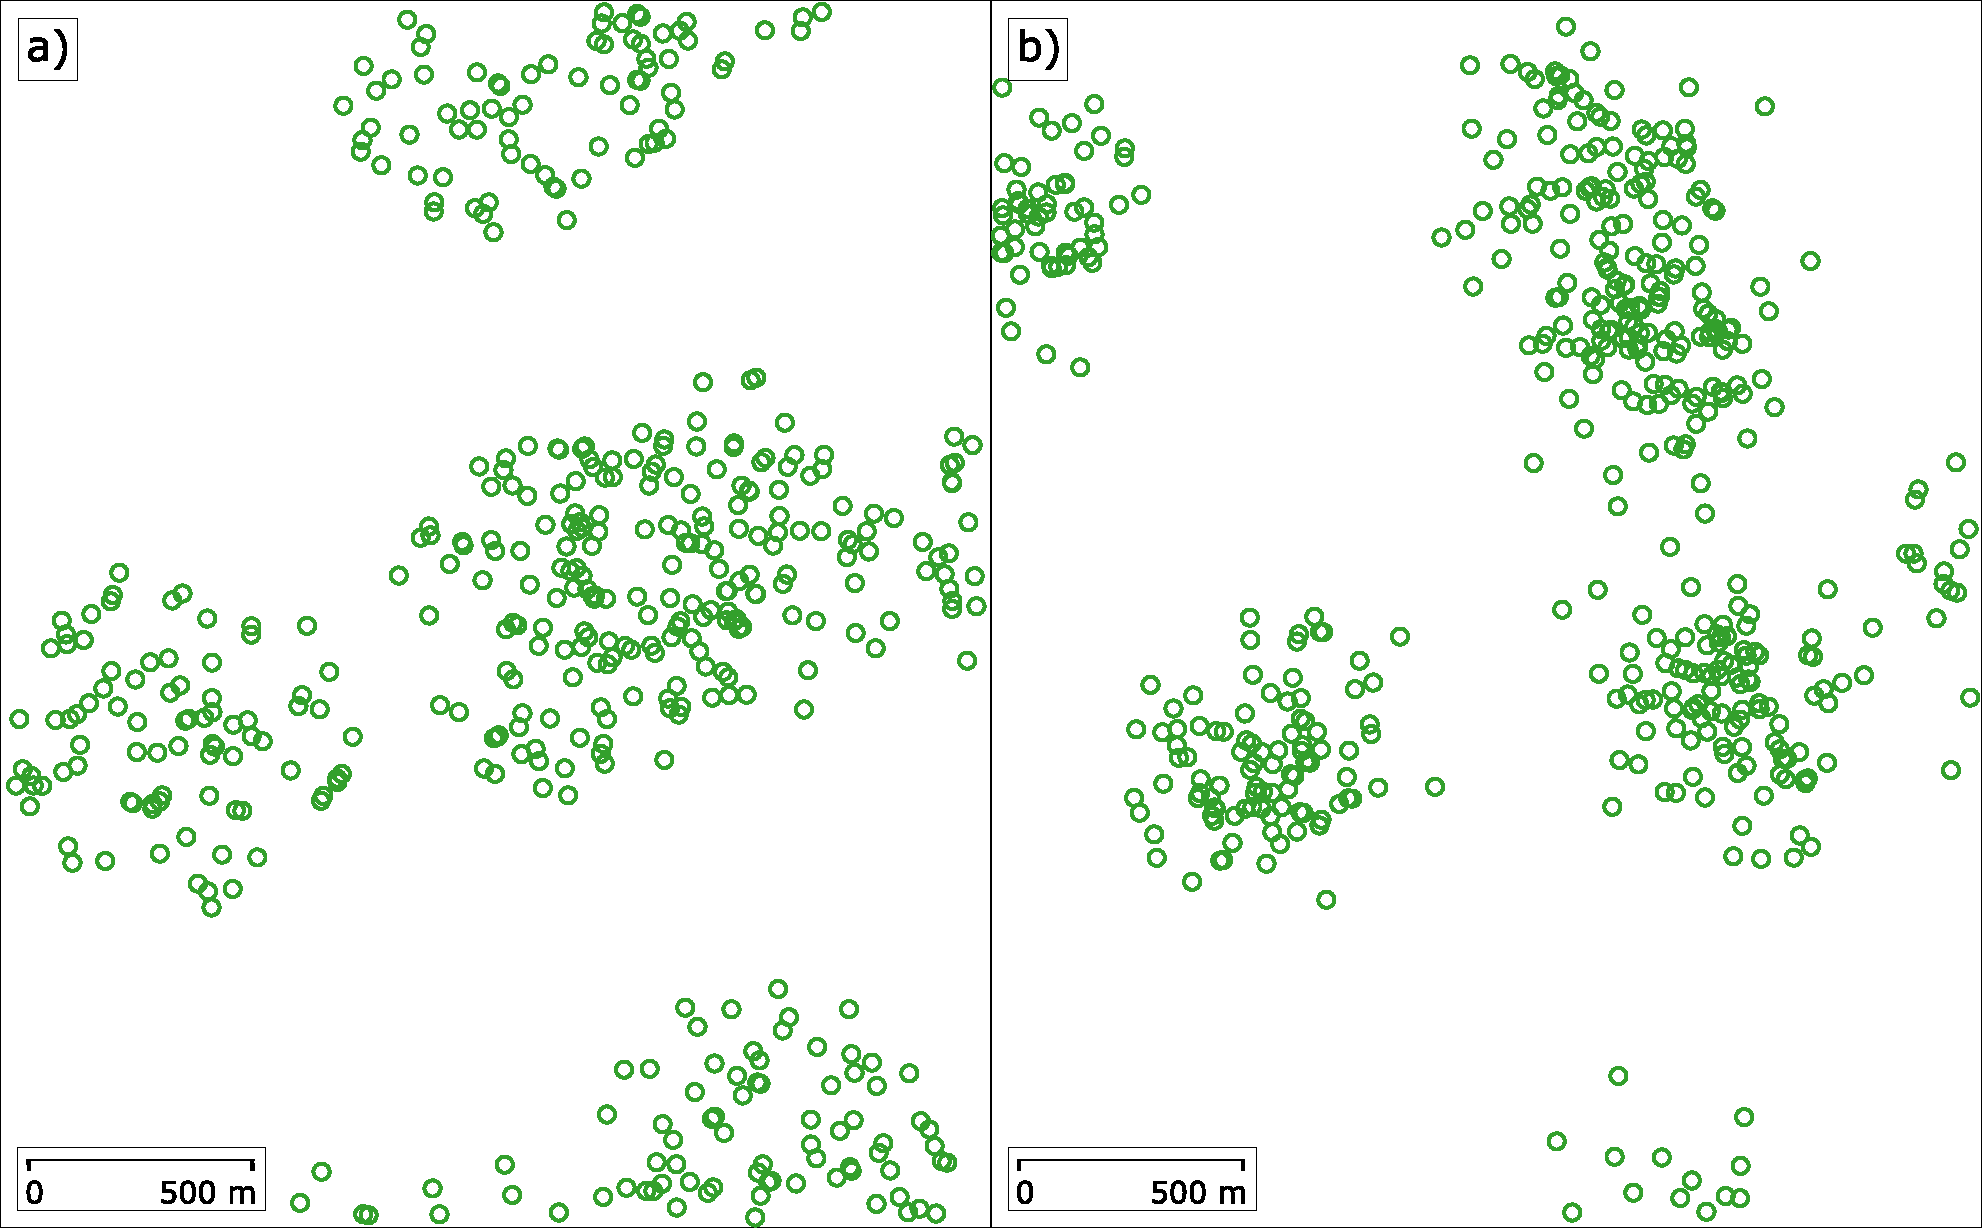
\includegraphics[width=\textwidth]{figures/Figure1.pdf}
    \caption[Beispielabbildung]{Dies ist eine Beispielabbildung. Die Optionen b und t geben an, dass der LaTeX-Compiler zunächst versuchen soll, die Graphik am unteren Rand zu positionieren (bottom). Falls das nicht möglich ist, soll sie am oberen Rand platziert werden (top). Selbstverständlich kann diese Reihenfolge auch umgedreht werden. Die Option gäbe die Platzierung auf einer eigenen Seite an. Der Eintrag in den eckigen Klammern vor dieser Bildunterschrift erscheint im Abbildungsverzeichnis.}
    \label{fig:1}
\end{figure}

\begin{figure}[tbp]
\centering
\subfloat[Moran drop plot for $\alpha = 0.01$ and binary spatial contiguity weights with C-normalisation]{%
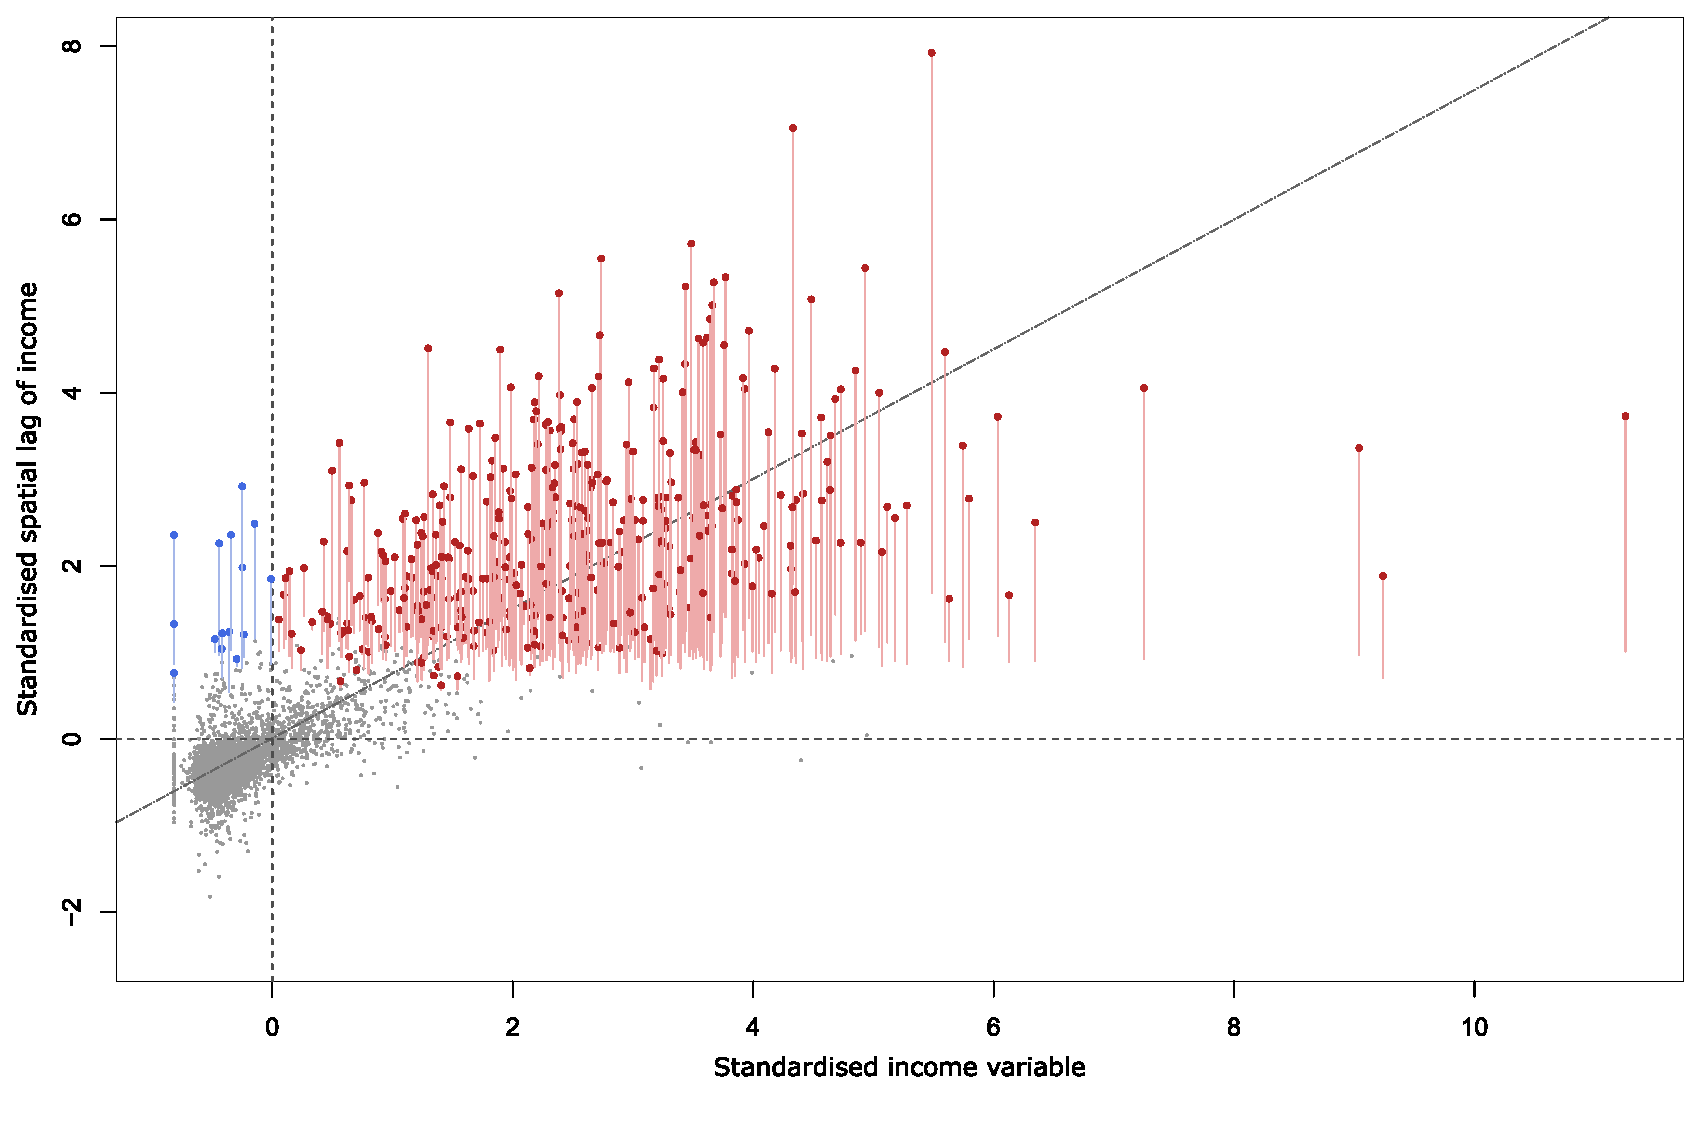
\includegraphics[height=8.5cm]{figures/Figure2a.eps}}\\
\subfloat[Moran drop plot for $\alpha = 0.01$ and binary spatial contiguity weights with W-normalisation]{%
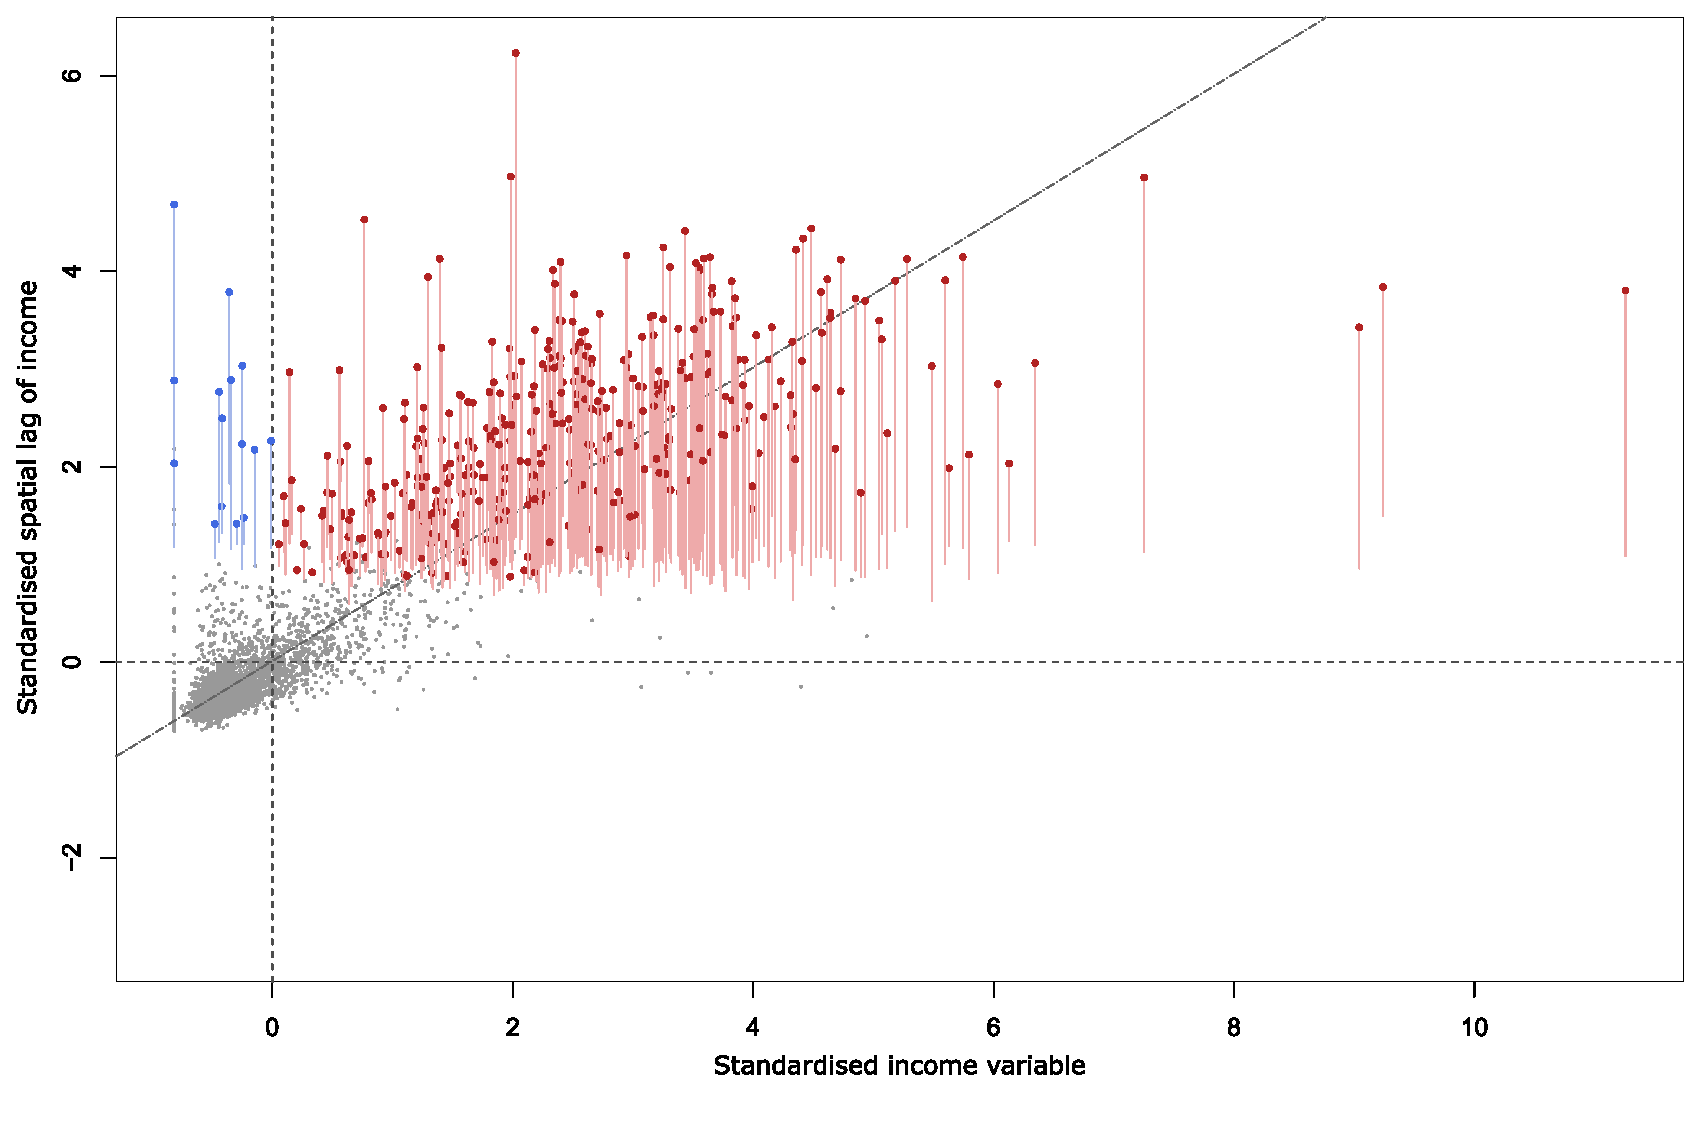
\includegraphics[height=8.5cm]{figures/Figure2b.eps}}
\caption{Moran drop plots on top of Moran scatterplots. Drop lines show the distances of significant values (points) from their critical values for positive (red) and negative (blue) autocorrelation.} \label{fig:2}
\end{figure}

Einen neuen Absatz erzeugt man einfach durch eine Leerzeile. Dieser Absatz wird dann in der ersten Zeile eingerückt. Im Folgenden findet sich ein Lorem-Ipsum-Beispieltext, damit hier irgendwas los ist. Natürlich sollte ein Absatz länger sein, als dieser kurze zweite Absatz.

\lipsum[1-20]